\documentclass[a4paper, 12pt]{article}%тип документа

%отступы
\usepackage[left=2cm,right=2cm,top=2cm,bottom=3cm,bindingoffset=0cm]{geometry}

%Русский язык
\usepackage[T2A]{fontenc} %кодировка
\usepackage[utf8]{inputenc} %кодировка исходного кода
\usepackage[english,russian]{babel} %локализация и переносы

%Вставка картинок
\usepackage{wrapfig}
\usepackage{graphicx}
\graphicspath{{pictures/}}
\DeclareGraphicsExtensions{.pdf,.png,.jpg}

%оглавление
\usepackage{titlesec}
\titlespacing{\chapter}{0pt}{-30pt}{12pt}
\titlespacing{\section}{\parindent}{5mm}{5mm}
\titlespacing{\subsection}{\parindent}{5mm}{5mm}
\usepackage{setspace}

%Графики
\usepackage{multirow}
\usepackage{pgfplots}
\pgfplotsset{compat=1.9}

%Математика
\usepackage{amsmath, amsfonts, amssymb, amsthm, mathtools}

%Стиль страницы
\usepackage{fancyhdr}
\pagestyle{fancy}

\begin{document}

\begin{titlepage}

\begin{center}
%\vspace*{1cm}
\large\textbf{Московский Физико-Технический Институт}\\
\large\textbf{(национальный исследовательский университет)}
\vfill
\line(1,0){430}\\[3mm]
\huge\textbf{Лабораторная работа №4.3.3}\\
\large\textbf{Исследование разрешающей способности микроскопа методом Аббе}\\
\line(1,0){430}\\[1mm]
\vfill
\large Баканова К.В., Б01-003\\
%\vspace*{1cm}
\large апрель 2022 г.\\
\end{center}

\end{titlepage}
\fancyhead[R] {Лабораторная работа №4.3.3}
\fancyhead[L] {Баканова К.В.}
\textbf{Цель работы}: определение дифракционного предела разрешения объектива микроскопа.

\textbf{       }

\textbf{В работе используются}: лазер; кассета с набором сеток разного периода; щель с микрометрическим винтом; оптический стол с набором рейтеров и крепёжных винтов; экран; линейка.

\textbf{       }

\section*{Теория}
\fancyhead[R] {Лабораторная работа №4.3.3}
\fancyhead[L] {Баканова К.В.}

Для иммерсионного микроскопа разрешающая способность объектива при \textit{некогерентном} освещении
\begin{equation}
\ell_{min} \approx \dfrac{0.61\lambda}{n \sin u},
\end{equation}
где $u$ -- апертурный угол объектива микроскопа (угол между оптической осью и лучом, направленным из центра объекта в край линзы).

\textbf{       }

Метод Аббе для оценки разрешающей способности состоит в разделении хода хучей на две части: сначала рассматривается картина в задней фокальной плоскости $F$ объектива -- она называется \textit{первичным изображением} или \textit{фурье-образом}. Это первичное изображение рассматривается как источник волн (принцип Гюйгенса-Френеля), создающий изображение в плоскости $P_2$, сопряжённой плоскости предмета -- \textit{вторичное изображение}.\\
Первичное изображение есть картина дифракции Фраунгофера (на дифракционной решётке), если её период $d$, то для направления максимальной интенсивности $\varphi_m$

\textbf{       }

	\textbf{Разрешающей способностью оптического прибора} называют минимальное расстояние $l_{\text{min}}$ между двумя точками в пространстве предметов, которое прибор может разрешить. Если наблюдения с помощью микроскопа ведутся при внешнем освещении, то, как правило, различные точки предмета рассеивают когерентные волны. Теория разрешающей способности для случая освещаемых объектов была разработана Аббе.

	Рассмотрим когерентно освещенный объект, наблюдаемый в объектив микроскопа. Минимальное разрешаемое объективом расстояние определяется условием
	\begin{equation}
		\label{min}
		l_{\text{min}} \approx \frac{\lambda}{\sin A} \approx \frac{\lambda}{D/2f},
	\end{equation}
	где $A$ -- апертурный угол микроскопа, $D$ -- диаметр диафрагмы. При этом диафрагма, расположенная симетрично, пропускает нулевой и $\pm 1$ дифракционные максимумы.
	
	В нашей работе применяется двумерная решётка -- сетка. В таком случае главные максимумы возникают тогда, когда одновременно выполняются условия:
	\begin{equation}
		\label{system}
		\begin{cases}
			d \sin \theta_x = m_x \lambda, \\
			d \sin \theta_y = m_y \lambda,
		\end{cases}
	\end{equation}
	где $m_x$ и $m_y$ -- целые числа, харакетризующие порядки дифракционных максимумов, $\theta_x$ и $\theta_y$ -- направления нв главные дифракционные максимумы в горизонтальное и вертикальной плоскостях соответственно.
	
	Максимумы, удовлетворяющие условию $\theta_x, \theta_y < A$, создают в задней фокальной плоскости $F$ объектива картину дифракции Фраунгофера  -- первичное изображение:
	
	\begin{figure}[h]
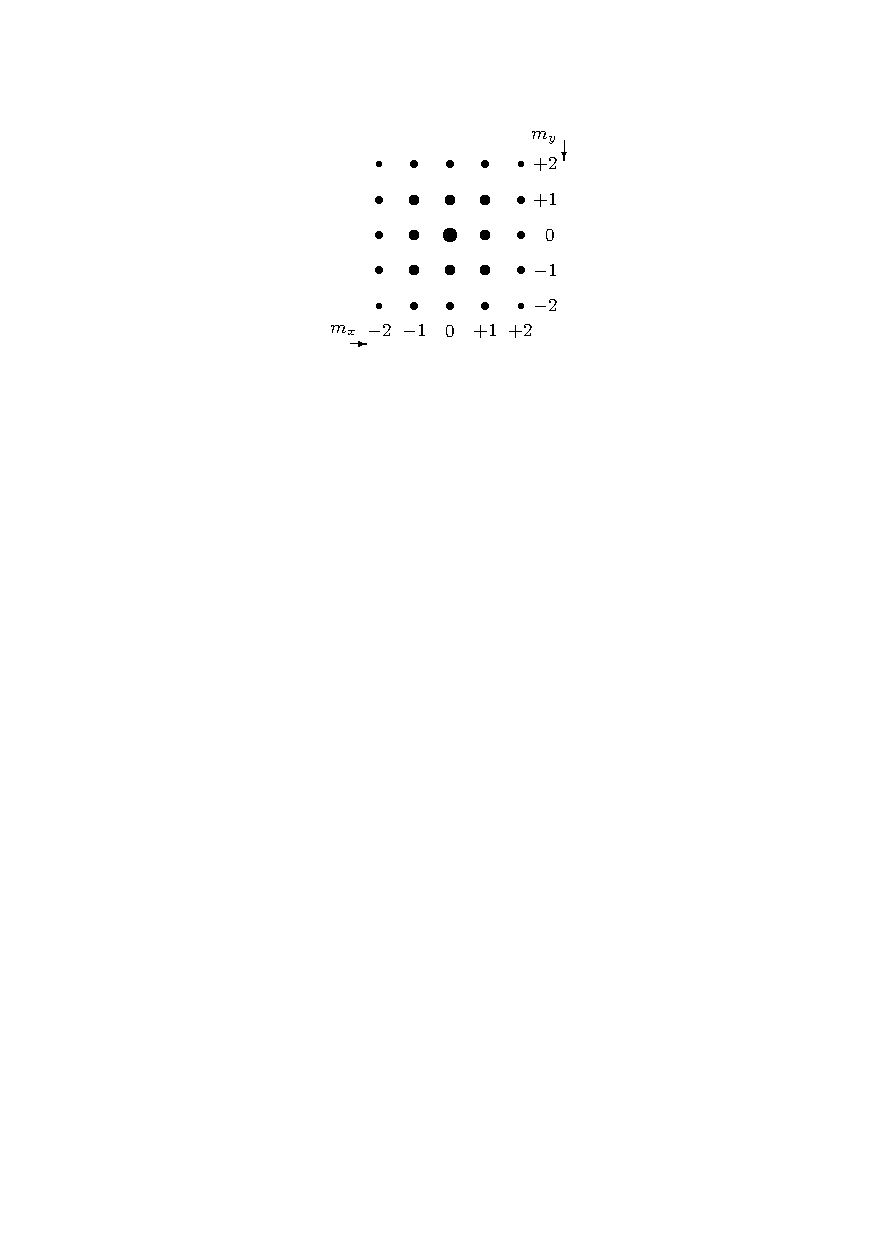
\includegraphics[scale=1.5]{max.pdf}
\centering
\caption{Дифракция Фраунгофера на двумерной решётке (сетке). Максимумы изображены кружками, размеры которых характеризуют интенсивности.}
\end{figure}
	
	Если теперь поместить в фокальной плоскости щель так, чтобы через неё проходили дифракционные максимумы с $m_x = 0$ и $m_y =0, \pm 1, \pm 2, ...$ (с $m_y = 0$ и $m_x =0, \pm 1, \pm 2, ...$), то в плоскости $P_2$ получится изображение решётки с горизонтальными (вертикальными) штрихами. Таким образом можно продемонстрировать явление \textit{пространственной фильтрации} -- выделение различных структур в изображении.




\section*{Экспериментальная установка}
\begin{figure}[h]
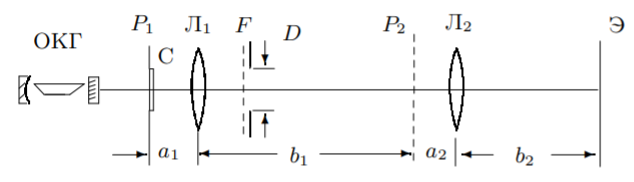
\includegraphics[scale=0.9]{1.png}
\centering
\caption{Схема установки.}
\centering
\end{figure}
Схема установки приведена на Рис. 1. Предметом $P_1$ служат сетки в кассете $C$. Линза $\text{Л}_1$ длиннофокусная, а $\text{Л}_2$ короткофокусная. В $F$ устанавливаются диафрагмы $D$, с помощью сеток с разными $d$ и щелевой диафрагмы можно проверить соотношение (3). Период сеток может быть измерен либо по расстоянию между дифракционными максимумами на экране, либо по увеличенному с помощью микроскопа изображению сетки на экране. Пространственную фильтрацию (получение наклонного изображение решётки) можно получить с помощью подбора угла наклона и ширины вспомогательной щели.

\textbf{       }

\section*{Ход работы}
\subsection*{1. Определение периода решёток по их пространственному спектру}
\fancyhead[R] {Лабораторная работа №4.3.3}
\fancyhead[L] {Баканова К.В.}
Соберём установку согласно Рис 1, за исключением линз. Длина волны излучения лазера $\lambda = 532 \text{ нм}$.\\
\textbf{       }

Расстояние от сетки до экрана $H = 141 \pm 2 \text{ см}$.\\
\textbf{       }

Измерим линейкой на экране расстояние $\Delta x$ между $n+1$ максимумами и рассчитаем по формуле (2) с учётом $\varphi = \frac{\Delta x}{H}$ период решётки $d = \frac{n \lambda}{\Delta x}H$, на основании данных построим таблицу:
\begin{table}[h]
\begin{tabular}{|c|c|c|c|c|c|}
\hline
Реш. & $\Delta x$ см & $\sigma_{\Delta x}$, см & $n$  & $d$, мкм & $\sigma_d$, мкм \\ \hline
1     & 22.7         & 0.1                   & 6  & 20 & 3        \\ \hline
4     & 22.6         & 0.1                   & 9  & 30 & 3        \\ \hline
3     & 25.1         & 0.1                   & 20 & 60 & 3        \\ \hline
4     & 22.5         & 0.1                   & 35 & 117 & 3 	\\ \hline
5     & 22.7         & 0.1                   & 48 & 159 & 4        \\ \hline
\end{tabular}
\centering
\caption{Метод 1 по нахождению периодов решёток.}
\end{table}\\
Погрешность $d$ считаем по формуле:
\textbf{       }

$$
\sigma_{d} = \sqrt{\left(\dfrac{\partial d}{\partial \Delta x}\right)^2 \sigma^2_{\Delta x} + \left(\dfrac{\partial d}{\partial n}\right)^2 \sigma^2_{n} + \left(\dfrac{\partial d}{\partial \Delta x}\right)^2 \sigma^2_{H}} =\lambda \sqrt{\dfrac{n^2 H^2 \sigma^2_{\Delta x}}{\Delta x^4} + \dfrac{\Delta x^2 \sigma^2_{n} \sigma^2_{H}}{n^2} + \dfrac{H^2 \sigma^2_{n}}{\Delta x^2}}.
$$

\textbf{       }

\subsection*{2. Определение периода решёток по изображению, увеличинному с помощью микроскопа}
\fancyhead[R] {Лабораторная работа №4.3.3}
\fancyhead[L] {Баканова К.В.}
Соберём модель микроскопа, добавив линзы согласно Рис. 1. Фокусные расстояния линз $F_1 = 110 \text{ мм}$, $F_2 = 25 \text{ мм}$. Измеряем необходимые расстояния:
$$
\begin{array}{r}
a_1 = 120 \pm 10 \text{ мм},\\
a_2 + b_1 = 455 \pm 10 \text{  см},\\
b_2 = 815 \pm 10 \text{ см},
\end{array}
$$
Из формулы тонкой линзы $a_2 = \frac{b_2 F_2}{b_2 - F_2} = 25.79 \text{ мм}$, откуда $a_2 \approx F_2$, поэтому в дальнейшем будем использовать это значение, следовательно $b_1 = 420 \pm 10 \text{ мм}$. \\
\textbf{       }

Увеличение микроскопа $\Gamma = \dfrac{b_1 b_2}{a_1 a_2} = 114 \pm 10$. Погрешность находится по формуле
$$
\sigma_\Gamma = \sqrt{\left(\dfrac{\partial \Gamma}{\partial a_1}\right)^2 \sigma^2_{a_1} + \left(\dfrac{\partial \Gamma}{\partial b_1}\right)^2 \sigma^2_{b_1} + \left(\dfrac{\partial \Gamma}{\partial b_2}\right)^2 \sigma^2_{b_2}}.
$$
\textbf{       }

Повторим измерения периодов изображений в новой конфигурации, погрешности считаются аналогично, полученные данные занесем в таблицу:

\begin{table}[h]
\begin{tabular}{|c|c|c|c|c|c|}
\hline
Реш. & $\Delta x$, см & $\sigma_{\Delta x}$, см & $n$ & $d$, мкм & $\sigma_d$, мкм \\ \hline
1     & 3.7            & 0.1                     & 16  & 20       & 2               \\ \hline
2     & 15.7           & 0.1                     & 49  & 28       & 3               \\ \hline
3     & 25.3           & 0.1                     & 38  & 58       & 5               \\ \hline
4     & 24.1           & 0.1                     & 18  & 117      & 12              \\ \hline
5     & 23.6           & 0.1                     & 13  & 159      & 19              \\ \hline
\end{tabular}
\centering
\caption{Метод 2 по нахождению периодов решёток..}
\end{table}\\

Здесь $d$ определялось по формуле $d = \dfrac{\Delta x}{\Gamma n}$
погрешность $d$:
$$
\sigma_d = \sqrt{\left(\dfrac{\partial d}{\partial \Delta x}\right)^2 \sigma^2_{\Delta x} + \left(\dfrac{\partial d}{\partial n}\right)^2 \sigma^2_{n} + \left(\dfrac{\partial d}{\partial \Gamma}\right)^2 \sigma^2_{\Gamma}}.
$$
\textbf{       }

Обратим внимание, что значения периодов решётки совпадают в пределах погрешности.

\textbf{       }

\subsection*{3. Определение периода решёток по оценке разрешающей способности микроскопа}
\fancyhead[R] {Лабораторная работа №4.3.3}
\fancyhead[L] {Баканова К.В.}
Поместим в фокальной плоскости линзы $\text{Л}_1$ щелевую диафрагму с микрометрическим винтом и определим минимальную толщину $D$ при которой на экране видна двумерная решётка. В этом случае период будет вычисляться по формуле (3) в предельном случае
$$
d = \dfrac{2\lambda F_1}{D},
$$
погрешность вычисляется по формуле 
$$
\sigma_d = d \dfrac{\sigma_D}{D}.
$$
Результаты приведены в Таблице 3.
\textbf{       }

\begin{table}[h]
\begin{tabular}{|c|c|c|c|}
\hline
D, мм & $\sigma_D$, мм & $d$, мкм & $\sigma_d$, мкм \\ \hline
4.14  & 0.02           & 28.27    & 3            \\ \hline
1.960 & 0.010          & 59.7     & 3             \\ \hline
1.020 & 0.010          & 114.7    & 3             \\ \hline
0.810 & 0.010          & 144.5    & 4             \\ \hline
\end{tabular}
\centering
\caption{Метод 3 по нахождению периодов решёток.}
\end{table}\\
\textbf{       }

Через щель проходили только нулевой (по центру) и два первых максимумы, за исключением второй щели, где нулевой максимум был помещён к краю щели. Для первой решётки период таким методом измерить не получилось, так как ширины щели не хватает.
\begin{figure}[h]
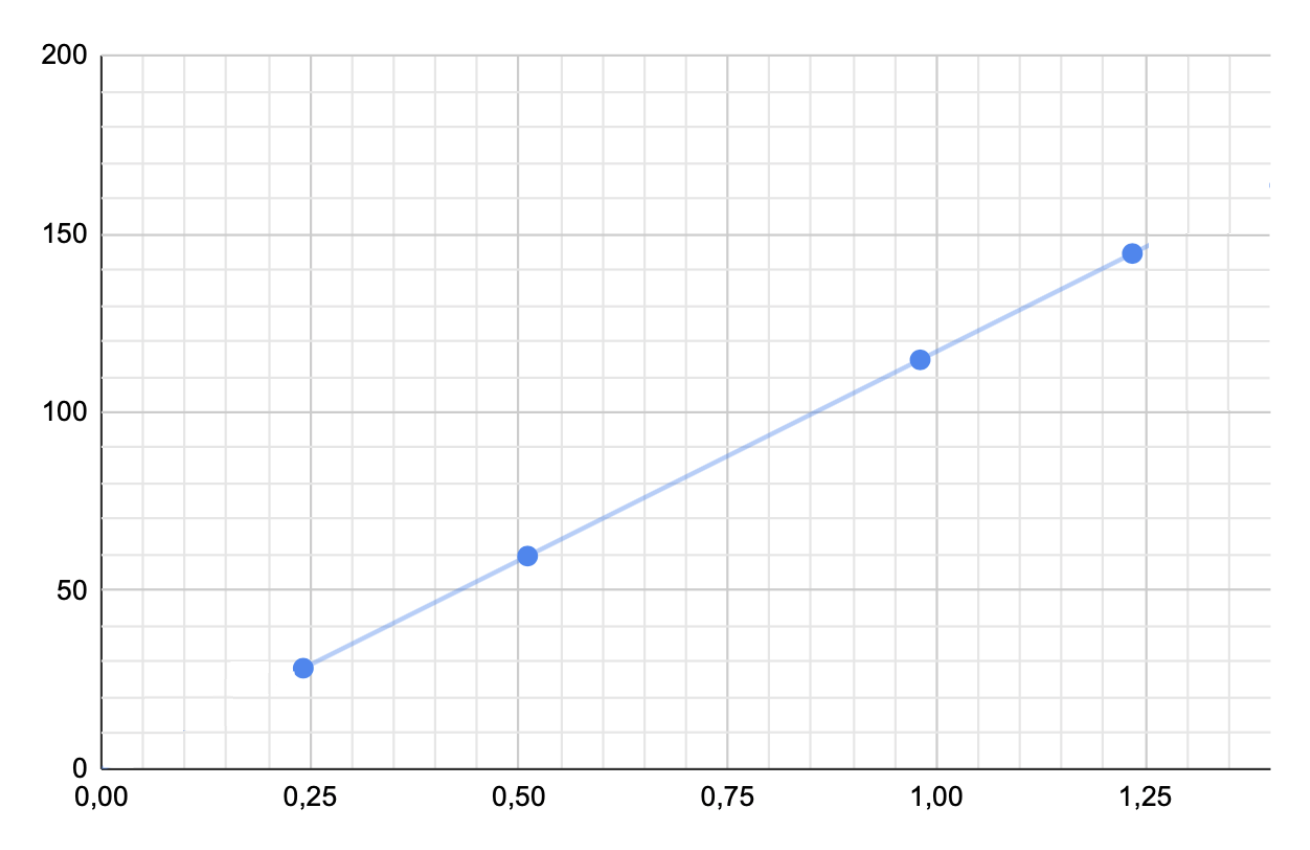
\includegraphics[scale=0.7]{2.png}
\centering
\caption{Зависимость $d = f(1/D)$.}
\end{figure}
\textbf{       }

Для проверки теории Аббе построим график $d = f(\frac{1}{D})$ со значениями $d$ из части 1, погрешность $\frac{1}{D}$ рассчитывается по формуле
$$
\sigma_{1/D} = \dfrac{\sigma_D}{D^2}.
$$
Угловой коэффициент прямой из МНК $k = (124 \pm 8) \cdot 10^{-9} \text{ м}^2$, в пределах погрешности он совпадает с теоретическим $2\lambda F_1 = 117 \cdot 10^{-9} \text{ м}^2$. Таким образом, теория Аббе подтвердилась.
\begin{table}[h]
\begin{tabular}{|c|c|c|c|c|}
\hline
Реш. & $1/D$, $\text{мм}^1$ & $\sigma_{1/D}$, $\text{мм}^1$ & $d$, мкм & $\sigma_d$, мкм \\ \hline
2    & 0.2415               & 0.0012                        & 30       & 3               \\ \hline
3    & 0.5100                & 0.0030                         & 60       & 3               \\ \hline
4    & 0.9800                & 0.0100                         & 117      & 3               \\ \hline
5    & 1.2350                & 0.0150                         & 159      & 4               \\ \hline
\end{tabular}
\centering
\caption{Значения для графика $d = f(1/D)$.}
\end{table}

\textbf{       }

\subsection*{4. Пространственная фильтрация и мультиплицирование}
\fancyhead[R] {Лабораторная работа №4.3.3}
\fancyhead[L] {Баканова К.В.}
Для наблюдения фильтрации на сетке 2 откроем щель так, чтобы она пропускала только максимум нулевого порядка и, поворачивая щель, наблюдаем за изменением картины.
Для наблюдения мультиплицированния поменяем местами сетку и щель, пронаблюлюдаем мультипликацию.
\textbf{       }

\section*{Вывод}
	В ходе данной лабораторной работы мы определили периоды дифракционных решёток различными способами. Полученные результаты отличаются друг от друга существуенно (наименьший от наибольшего в два раза), хотя имеют одинаковый порядок величины. Это может быть связано с приближенным характером используемой теории, неточностью определения величин $a_2$ и $b_1$, неисправностью источника света, который в ходе выполнения лабораторной работы периодически выключался. 
	
	Стоит отметить, что у всех величин, полученных прямым измерением, мы принебрегли случайной погрешностью, так как она мала по сравнению с систематической, которая явным образом повлияла на разброс результатов.
	
	Не смотря на расхождения, нам удалось убедиться в справедливости формулы, то есть проверка теории Аббе оказалась положительной. Действительно, периоды решёток, определенные в первом и третьем способах, отличаются от их среднего значения на 20 \%, что может навести на мысль о том, что во втором способе, скорее всего, имеется грубая ошибка и эксперимент требует повторного проведения.
	
	Выход из строя источника света не позволил пронаблюдать за явлениями фильтрации и мультиплицирования.



\end{document}
